%!TEX root = ../thesis.tex
%*******************************************************************************
%*********************************** First Chapter *****************************
%*******************************************************************************


\chapter{Markov Processes}  %Title of the First Chapter

\ifpdf
    \graphicspath{{Chapter1/Figs/Raster/}{Chapter1/Figs/PDF/}{Chapter1/Figs/}}
\else
    \graphicspath{{Chapter1/Figs/Vector/}{Chapter1/Figs/}}
\fi


%********************************** %First Section  **************************************
\section{Markov Processes} %Section - 1.1 

In order to fully understand and explore the properties and implications of Hidden Markov Models (hereinafter "HMMs") that will be used for cryptocurrency price prediction it is necessary to apriori state the underlying definition of Markov processes imminently followed by Markov Chains and finally Hidden Markov Models. 

\subsection{Definition and Properties}

Definition. Given a measurable space (S, B) called state space, where S is
a set and B is a {sigma}-algebra on S. A function P : S × B → R is called a
transition probability function if P(x, ·) is a probability measure on (S, B)
for all x  S and if for every B  B, the map s → P(s, B) is B-measurable.
Define P
1
(x, B) = P(x, B) and inductively the measures P
n+1(x, B) =
R
S
P
n(y, B)P(x, dy), where we write R








\nomenclature[z-cif]{$CIF$}{Cauchy's Integral Formula}                                % first letter Z is for Acronyms 
\nomenclature[a-F]{$F$}{complex function}                                                   % first letter A is for Roman symbols
\nomenclature[g-p]{$\pi$}{ $\simeq 3.14\ldots$}                                             % first letter G is for Greek Symbols
\nomenclature[g-i]{$\iota$}{unit imaginary number $\sqrt{-1}$}                      % first letter G is for Greek Symbols
\nomenclature[g-g]{$\gamma$}{a simply closed curve on a complex plane}  % first letter G is for Greek Symbols
\nomenclature[x-i]{$\oint_\gamma$}{integration around a curve $\gamma$} % first letter X is for Other Symbols
\nomenclature[r-j]{$j$}{superscript index}                                                       % first letter R is for superscripts
\nomenclature[s-0]{$0$}{subscript index}                                                        % first letter S is for subscripts


%********************************** %Second Section  *************************************
\section{Discrete-time Markov Chains} %Section - 1.2

Let $\Omega \neq \emptyset$ and $A \subseteq 2^{\Omega}$ be a $\sigma$-algebra on $\Omega$, and $P$ a measure on A with $P(\Omega) = 1$, i.e. $P$ is a {\it probability measure}. Then the triplet $(\Omega, A, P)$ is called a {\it probability space}. Where $\Omega$ denotes a sure event and it holds that $\forall \omega \in \Omega$ is called an elementary event. Furthermore, $\forall A \in A$ is a random event  so that $P(A)$ is a probability of such a random event. 

Let $I$ be a countable set and $\Theta$ a $\sigma$-algebra on $I$. Each $i \in I$ is called a {\it state} and $(I,\Theta)$ a {\it state-space}. We say that $\lambda = (\lambda_i : i \in I) $ is a measure on I if $0 \leq \lambda_i \leq \infty$. If in addition the {\it total mass} $\sum_{i \in I} \lambda_i = 1$ then $\lambda$ is a {\it distribution} (or probability measure). 

Suppose now that we have two measurable spaces $(\Omega,A)$ and $(I,\Theta)$ and a random variable $X: \Omega \rightarrow I$ assuming that X is measurable. Thus we call $(I,\Theta)$ a state space and $(\Omega, A)$ an underlying space. Therefore we may set:

\begin{equation}
\lambda_X(i) = P(X=i)=P(\{\omega: X(\omega)=i\})
\end{equation}

Since we are allowing only for the discrete realisations of the random variable X, given previous assumptions, $\lambda_X(i)$ is a {\it probability mass function}.

Then measure $\lambda$ defines a distribution of $X$. Given such a setting random variable $X$ is assumed to denote random state $i$ with probability $\lambda_i$. 

To simply illustrate the idea behind discrete Markov Chains let us assume a situation where the future market movements transition between a countable number of states $I =$ \{upward movement, no movement, downward movement\} and there is a transition matrix (also called {\it stochastic matrix}) $P = (p_{i,j} : i,j \in I)$ defined as:
\begin{equation*}
P =
\begin{pmatrix}
0.1 & 0.4 & 0.5 \\
0.25 & 0.3 & 0.45 \\
0.33 & 0.33 & 0.33 
\end{pmatrix}
\end{equation*}
Each row represents full set of transition probabilities between each state which is visible from $\sum_{j \in I} ^{}p_{i,j} = 1 $, i.e. each row of matrix $P$ represents a full distribution of transitions over $I$. Such a relationship can be represented as a diagram indexing each state by A, B and C respectively as follows:

\begin{center}
\begin{tikzpicture}[->, >=stealth', auto, semithick, node distance=3cm]
\tikzstyle{every state}=[fill=white,draw=black,thick,text=black,scale=1]
\node[state]    (A)                     {$A$};
\node[state]    (B)[right of=A]   {$B$};
\node[state]    (C)[right of=B]   {$C$};

\path
(A) edge[loop left]     node{$0.1$}         (A)
    edge[bend left,below]     node{$0.4$}     (B)
    edge[bend right,below]      node{$0.5$}      (C)
(B) edge[bend left,below]     node{$0.45$}           (C)
    edge[loop below]     node{$0.3$}           (B)
    edge[bend left, above]     node{$0.25$}           (A)
(C) edge[bend right,above] node{$0.33$}           (A)
    edge[loop right]     node{$0.33$}         (C)
    edge[bend left, above]      node{$0.33$}         (B);
\end{tikzpicture}
\end{center}
 
This may be easily interpreted for each given state. For example if we assume that the market moved upwards on the last trading day there is a 0.1 chance that the market will move in positive direction today, in other words the conditional probability of observing the state A today given the state A yesterday is 0.1. On the hand if we suppose that today the market actually transitioned to the state B  with probability 0.4 there is now a probability of 0.45 to transition to state C since the future transition is only conditioned by its previous state. 

Till now we have assumed random variable X that modelled the probability of observing a state $i \in I$ given the initial distribution $\lambda$. We ought to consider  thus we have to allow for a system of discrete random variables that are also identically distributed for each time step $\{X_{t},t \in T \}$, for $\{t_0,t_1,...,t_n\} \subset T$ where $n \in \mathbb{N}_0$.

Suppose now that we have observed a given sequence of states for the last week as $\{A,B,C,C,A\}$ and we would like to know its probability of observing given the transition matrix P and distribution $\lambda$. Then $P(X_{t_0},...,X_{t_n}|P,\lambda)$ can be calculated as:

\begin{align*}
P(X_{t_0},...,X_{t_n}|P,\lambda) &= P(A,B,C,C,A|P,\lambda) \\
&= P(A) * P(B|A) * P(C|B) * P(C|C) * P(A|C) \\
&= \lambda * p_{1,2} * p_{2,3} * p_{3,3} * p_{3,1} \\
&= \lambda * 0.4 * 0.45 * 0.33 * 0.33
\end{align*}

maybe bych tam dal product of Xs

Where the probability of observing state A is determined by our distribution $\lambda$ evaluated at respective state A since we have no prior knowledge about what exactly happened before $t_0$. 

On the other hand, we might consider a situation in which we have observed such a sequence of events and we need to determine the next state given the sequence. As in the last example, we have our transition matrix P, distribution $\lambda$ and a sequence of events observed until now $\{A,B,C,C,A\}$ for $t_{k-4},...,t_{k}$. Let us also assume that $t_{k+1}$ is a time of next event for which we are trying to determine its probability.

\begin{align}
P(X_{t_{k+1}}|X_{t_{k}},...,X_{t_{k-4}}) &= P(X_{t_{k+1}}|X_{t_{k}})
\end{align}

We know that last observed state was A which directs us straight to the first row of our transition matrix P since from the properties of Markov Processes (the process is memoryless) we know that the next state will depend solely on the present state so we can abstract from the given sequence of past states and focus only on $X_{t_{k}}$. Finally we may conclude that the most likely future state is C with probability of 0.5. 

Obviously, the probabilities in previous transition matrix P were imaginary and served only as a mere example of the main properties of Discrete-time Markov Chains. From now on we consider a dataset of BTC-USD daily close prices calculated my CoinMarketCap website from 5th March 2017 to 5th March 2022. FIrst of all we ought to make several assumptions about the data in order to apply the logic and properties of Markov Chains. 

Assumption 1: The close daily prices of BTC-USD trading pair are discrete, meaning that we only record prices at exactly 0:00 of each day since there are no closing hours of the major cryptocurrency exchanges. This assumption will be elevated in the next section with Continous-time Markov Chains.

Assumption 2: We will assume that future prices of Bitcoin depend only on their pre





Theorems:





%********************************** % Third Section  *************************************
\section{Continous-time Markov Chains}  %Section - 1.3 
\label{section1.3}

















Viterbi algorithm should, in its most general form, provide a solution to the maximum a posteriori probability (MAP) estimation of the state sequence of a finite-state discrete-time Markov process introduced in the last chapter. 


\section{Hidden Markov Model}

Up until now we have considered visible states in a sense that the sequence of states was known, we refer to these models as $visible$ $Markov$ $Models$. In this section we will consider a situation in which we do not observe the states directly but only as a guess given other visible observations that are available to us. These "visible" observations are considered as an emissions from the hidden state sequence. Thus, the observations are assumed to be generated by the hidden states. We may interpret this relation by the following diagram where we have a hidden state sequence $S = \{S_1, S_2,...S_T\}$:

\begin{figure}[h]

\begin{center}
	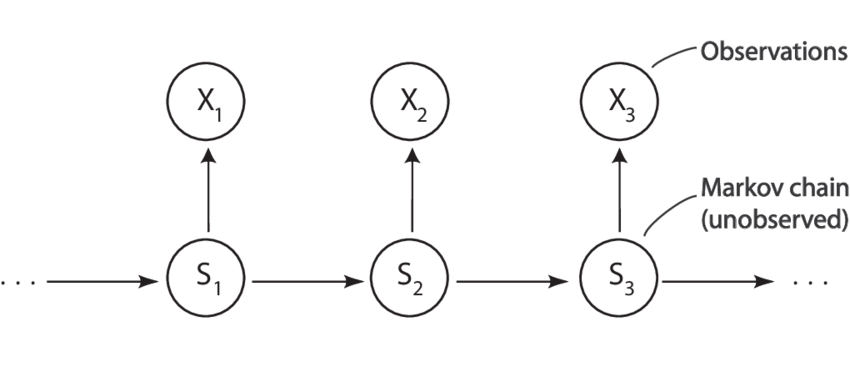
\includegraphics[width=0.7\textwidth]{States.png}
\end{center}

\caption{\textit{Simplified structure of the hidden Markov process with observable states $X_1,X_2,X_3$ and hidden states $S_1,S_2,S_3$}}

\end{figure}

There are 3 main assumptions of Hidden Markov Models as a consequence of the properties of Markov processes. For $Z = \{z_t\}_{t=0}^T$ being the hidden state sequence:

\begin{itemize}
\item[1)] The Markov assumption - this assumption states that the next hidden state $z_{t+1}$ depends only on the current state $z_t$, so that the transition probabilities are defined as:

\begin{equation}
P(z_{t+1} = j| z_{t} = i,z_{t-1} = l,...,z_{0} = n) = P(z_{t+1} = j| z_{t} = i) = p_{ij}
\end{equation}

It it also possible to assume that the states in HMM are dependant beyond the current state therefore giving rise to k-order HMMs as opposed to classical first-order HMM, moreover, such variations are uneasy to analyse.

\item[2)] The stationarity assumption - The transition matrix is invariant of the time, thus for any arbitrarily set time $t_1$ and $t_2$:

\begin{equation}
P(z_{t_1+1} = j| z_{t_1}) = P(z_{t_2+1} = j| z_{t_2} = i) = p_{ij}
\end{equation}

\item[3)] The observation independence assumption - The current observation or output is statistically independent of the previous observations. So if we have a observation sequence $X = \{x_1,x_2,...,x_T\}$ then:

\begin{equation}
P(X|z_1,z_2,...,z_T, \lambda) = \prod_{t=1}^T P(x_t|z_t,\lambda)
\end{equation}

\end{itemize}

Given these assumptions we define the joint probability of the hidden states and the observations $P(X,Z)$ as follows:

\begin{equation}
P(X, Z) = \prod_{t=1}^T P(z_t|z_{t-1}) P(x_t|z_t)
\end{equation}



There are mainly 3 fundamental problems in HMM that need to be resolved as in (Oliver C. Ibe):

\begin{itemize}
\item[1.] Evaluation problem - Given a model denoted as $\lambda = (P,\theta,\pi)$ and an observation sequence $X = x_1, x_2,...,x_T$, how to efficiently compute the probability that the model generated the observation sequence, in other words, what is $P(X|\lambda)$? 
\item[2.] Decoding problem - Given a model $\lambda = (P,\theta,\pi)$, what is the most likely sequence of hidden states that could have generated a given observation sequence? Thus we would like to find $Z = \underset{Z}{\arg\max} P(Z,X|\lambda)$, where $Z$ is the hidden state sequence. 
\item[3.] The learning problem - Given a set of observation sequences find the HMM that best explains the observation sequence. Thus, find the values of $\lambda$ that maximise $P(X|\lambda)$ or in order to estimate the most likely parameters of HMM for a given of observation sequence. 
\end{itemize}

The most traditional approaches in solving these 3 fundamental problems differ and one may not suffice in solving all three. The evaluation problem is usually by forward-backward algorithm, the decoding problem by well-known Viterbi algorithm and the last learning problem by Baum-Welsch algorithm which is a special case of Expectation-maximization (EM) algorithm. 


\subsection{Forward-backward algorithm}




\subsection{Viterbi algorithm}



\nomenclature[z-DEM]{DEM}{Discrete Element Method}
\nomenclature[z-FEM]{FEM}{Finite Element Method}
\nomenclature[z-PFEM]{PFEM}{Particle Finite Element Method}
\nomenclature[z-FVM]{FVM}{Finite Volume Method}
\nomenclature[z-BEM]{BEM}{Boundary Element Method}
\nomenclature[z-MPM]{MPM}{Material Point Method}
\nomenclature[z-LBM]{LBM}{Lattice Boltzmann Method}
\nomenclature[z-MRT]{MRT}{Multi-Relaxation 
Time}
\nomenclature[z-RVE]{RVE}{Representative Elemental Volume}
\nomenclature[z-GPU]{GPU}{Graphics Processing Unit}
\nomenclature[z-SH]{SH}{Savage Hutter}
\nomenclature[z-CFD]{CFD}{Computational Fluid Dynamics}
\nomenclature[z-LES]{LES}{Large Eddy Simulation}
\nomenclature[z-FLOP]{FLOP}{Floating Point Operations}
\nomenclature[z-ALU]{ALU}{Arithmetic Logic Unit}
\nomenclature[z-FPU]{FPU}{Floating Point Unit}
\nomenclature[z-SM]{SM}{Streaming Multiprocessors}
\nomenclature[z-PCI]{PCI}{Peripheral Component Interconnect}
\nomenclature[z-CK]{CK}{Carman - Kozeny}
\nomenclature[z-CD]{CD}{Contact Dynamics}
\nomenclature[z-DNS]{DNS}{Direct Numerical Simulation}
\nomenclature[z-EFG]{EFG}{Element-Free Galerkin}
\nomenclature[z-PIC]{PIC}{Particle-in-cell}
\nomenclature[z-USF]{USF}{Update Stress First}
\nomenclature[z-USL]{USL}{Update Stress Last}
\nomenclature[s-crit]{crit}{Critical state}
\nomenclature[z-DKT]{DKT}{Draft Kiss Tumble}
\nomenclature[z-PPC]{PPC}{Particles per cell}